\section{Implementing set computations}
\label{sec:implementing set computations}

\subsection{Transforming between $x$-space and $z$-space}
\label{sec:transforming x to z}
Let $\Xc \subset X$ be an arbitrary rectangular subset of $X$. 
The objective is to find $Z \subset \Re^{\dimX}$ s.t. $z \in  Z \implies \iT(x) \in \Xc$. 
Thus keeping the state $z$ of the linearized dynamics in $Z$ implies the nonlinear system's state $x$ remains in $X$.
We also need to find a subset $X_0 \subset X$ s.t. $T(X_0) \subset Z$, which will be used as our effective safe set for the $x$ dynamics.
This is needed for choosing bounds ??
\todo[inline]{is it? for choosing bounds on the v inputs, we need an over-approxiation of $ \iT(Z)$, not an under-approximatino. In fact we could use all of $X$ but that would be over-kill since we know that by forcing z in Z we are forcing x in $\iT(Z)$}
Because $T$ can be an arbitrary diffeomorphism this has to be implemented numerically.
In this section we provide such a procedure:
\begin{itemize}
	\item Let $Z_1 \subset \Re^{\dimX}$ be the rectangle with bounds in the $i^{th}$ dimension $[ \min_{x \in \Xc} T_i(x),  \max_{x \in \Xc} T_i(x) ]$, $i=1,\ldots, \dimX$.
	This over-approximates $T(\Xc)$. 
	Next we need to prune it so it under-approximates $T(\Xc)$. 
	\item Define $z_{in} \defeq \min \{ \|z \|_0 \such z \in Z_1, \iT(z) \notin \Xc\}$.
	$z_{in}$ is the smallest-norm inadmissible $z$ in $Z_1$.
	Thus all points in the $\ell_0$-ball of radius $\|z_{in}\|$ are admissible, i.e. their pre-images via $\iT$ are in $\Xc$.
	Now we need to get the $x$-set that maps to $B_z(0,\|z_{in}\|) \defeq B_{z}$  (or a subset of it).
	\item Let $X_1 \subset X$ be the rectangle with bounds in the $i^{th}$ dimension $[\min_{z \in B_{z}} \iT_i(z),  \max_{z \in B_{z}} \iT_i(z) ]$.
	Again, this is an over-approximation of $\iT(B_{z})$, so it needs to be pruned.
	\item Define $x_{in} = \inf \{\|x\|_0 \such x \in X_1, T(x) \notin B_{z}\}$.
	Then every point in the $\ell_0$-ball $B_x(0, \|x_{in}\|) \subset \Xc$ maps via $T$ to $B_{z}$
\end{itemize}
Therefore we choose $Z = B_z$ and $X_0 = B_x(0,  \|x_{in}\|)$.
%\subsection{Online reachability and overapproximation}
%As seen in Section \textbf{setdefs}, we need $X_{k}$ in order to compute the inner convex bound on the input $v$ at time $k$, $\underline{V}_k$, and also to compute the bounding set for the estimation error $\tilde{e}_k$, $\tilde{E}_k$. For our Robust Model Predictive Controller, we will need these sets for the length of the MPC horizon starting at time $k$, i.e. for time $k=0,\dotsc,N$. For the purpose of getting these sets for future inputs and estimation errors starting at time $k$, we compute an outer-approximation of the reachable sets for the non-linear system,  $\bar{X}_{k+j|k})$ starting at time $k$.
%
%For $j=0$, given the state estimate $\hat{x}_k$,  we have the set ${X}_{k|k}$ where the true state $X_k$ can lie, given as $X_{k|k} = \lbrace \hat{x}_k \rbrace \oplus (-E)$ since we know $\hat{x}_k = x_k + e_k$ and $e_k \in E$. Next, we compute the set of reachable states at time step $k+1$ starting from all states in ${X}_{k|k}$ and all inputs in $u \in U$. From this set, we make an over-approximation by adding (in the sense of Minkowsi Sum), $-E$ and $E$,  i.e. $\bar{X}_{k+1|k} = \text{Reach}_h(X_{k|k},U)\oplus(-E) \oplus(E)$. the reason for this over-approximation will become clearer later in this section. So for the sets in which $x_{k+j}$ can lie, given the state estimate at time $k$, we have $\forall j=0,\dotsc,N$
%\begin{subequations}
%\label{eq:overreach_NL}
%\begin{align}
%\bar{X}_{k|k}&=X_{k|k}=\lbrace\hat{x}_k\rbrace \oplus (-E) \\
%\bar{X}_{k+j|k}&=Reach_h(\bar{X}_{k+j-1},U) \oplus (-E) \oplus (E) \forall j=1,\dotsc,N
%\end{align}
%\end{subequations}
%
%We explain the reason behind the approximation via Figure \ref{fig:overreach_NL}. For $j>0$, we add (in the sense of Minkowski sum) $(-2E)$ to the set obtained via reachability in order to ensure that the over-approximated reachable sets computed for the same time instant $k+j$ at the next time step $k+1$ through Eq. \ref{eq:overreach_NL}, $\bar{X}_{k+j|k+1}$ are such that 
%
%\begin{equation}
%\label{eq:reach_contain}
%\bar{X}_{k+1+j|k+1} \subseteq \bar{X}_{k+1+j|k}
%\end{equation}
%
%Note, for time step $k+1$, $Reach_h(\bar{X}_{k|k},U)$ gives us the set where the actual state $x_k$ can lie. Since $\hat{x}_k = x_k+e_k$, $Reach_h(\bar{X}_{k|k},U) \oplus (E)$ gives us the set where the state estimate at time $k+1$, $\hat{x}_{k+1}$ can lie. Finally $Reach_h(\bar{X}_{k|k},U) \oplus (E) \oplus (-E)$ gives us a set in which $\lbrace \hat{x}_{k+1} \rbrace \oplus (-E)$, i.e. $\bar{X}_{k+1|k+1}$. At the next time step $k+2$, we similarly add $\oplus (-E)\oplus (E)$ to the set obtained from reachability on $\hat{X}_{k+1|k+1}$ becase we want the set computed at time $k+1$ via reachability on $\bar{X}_{k+1|k+1}$ to lie inside it and so on for other time steps. This gives us Eq. \ref{eq:reach_contain} $\forall k$ by following the reachability over approximations of Eq. \ref{eq:overreach_NL}.
%
%Given this approach, at time $k$, we have an over-approximation of the set in which $x_{k+j}$ lies for all $j=0,\dotsc,N$. These sets can be computed via online reachability algorithms in real-time, e.g. \textbf{RTReach}.
%
%\subsection{Computing bounding sets for $v$ and $\tilde{e}$ online}
%
%By computing the sets $\bar{X}_{k+j|k}$, we can use compute $\tilde{E}_{k+j}$ and $\underline{V}_{k+j}$ online using the definition of these sets. We have $\forall j=0,\dotsc,N$
%
%\begin{equation}
%\tilde{E}_{k+j|k}  = \cup_{x \in \bar{X}_{k+j|k}}M(x)E
%\end{equation}
%
%And, 
%
%\begin{equation}
%\underline{V}_{k+j|k} = \lbrace v|u\in U, \, \forall x \in \bar{X}_{k+j|k} \rbrace
%\end{equation}



\begin{figure*}
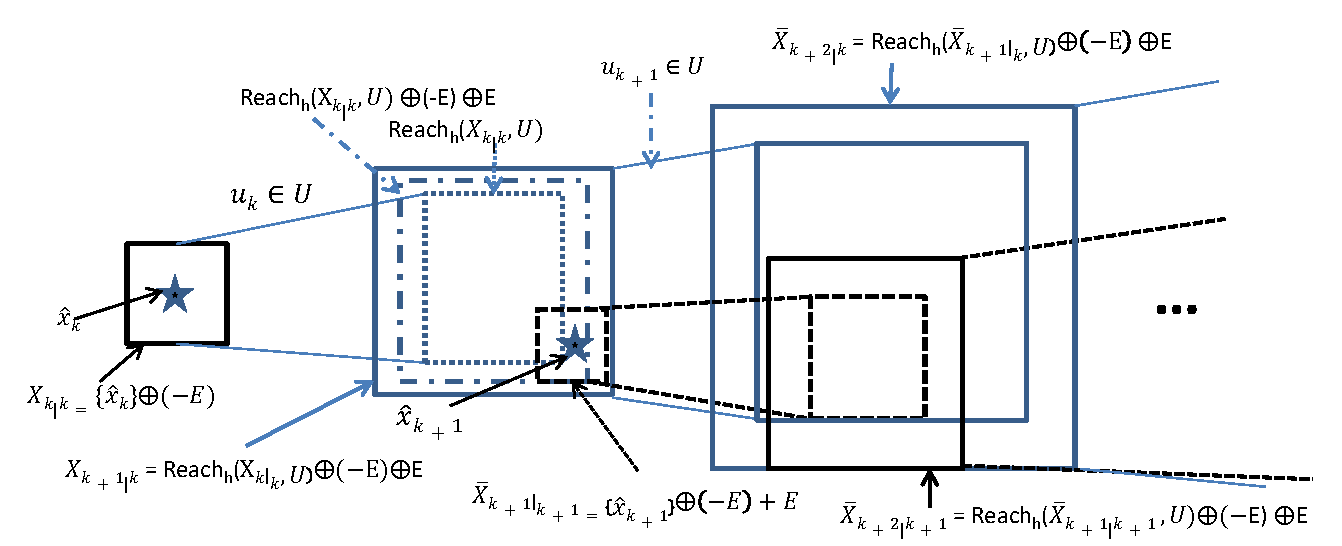
\includegraphics[scale=0.75]{figs/OverReachFigure_NL_scissored.pdf}
\caption{The over-approximated reachable sets for $x_{k+j}$, computed at time steps $k$, and correspondingly ay $k+1$ , used to compute $\tilde{E}_{k+j|k}$, $\underline{V}_{k+j|k}$. }
\label{fig:overreach_NL}
\end{figure*}